\documentclass[11pt]{article}
\usepackage[margin=1in]{geometry}
\usepackage{amsmath, amssymb}
\usepackage{enumitem}
\usepackage{tikz}
\usepackage{tikz-qtree}
\usetikzlibrary{arrows.meta, positioning, graphs, automata, matrix, calc}

\setlength{\parindent}{0pt}
\setlength{\parskip}{0.5em}
\setlist{nosep}

\tikzset{
    every tree node/.style={circle, draw, minimum size=0.6cm, inner sep=1pt},
    blank/.style={draw=none, fill=none, edge from parent/.style={draw=none}},
    blacknode/.style={circle, draw, fill=black, text=white, minimum size=0.6cm, inner sep=1pt},
    whitenode/.style={circle, draw, fill=white, text=black, minimum size=0.6cm, inner sep=1pt},
    rednode/.style={circle, draw, fill=white, text=black, minimum size=0.6cm, inner sep=1pt},
    tfnode/.style={rectangle, draw, rounded corners=2pt, minimum size=0.45cm, inner sep=1pt},
    listnode/.style={rectangle, draw, rounded corners=2pt, minimum height=0.6cm, inner sep=3pt},
    skipnode/.style={rectangle, draw, minimum size=0.6cm, inner sep=2pt},
    main node/.style={circle, draw, minimum size=0.6cm}
}
\begin{document}

\begin{center}
    \Large\textbf{CS 253: Data Structures and Algorithms}\\
    \large\textbf{Randomized Final Study Problem}
\end{center}
\vspace{1em}

% seed=1
% topic=huffman
% distinct_chars=7
% text_length=20
% distinct_code_lengths=3
% tied_weights=2
% huffman_bits=51
% fixed_bits=60

\section*{Greedy Algorithms}
\subsection*{Huffman Coding}
Consider the string \texttt{onongigohciigojgohoo} of length 20.

\begin{enumerate}[label=(\alph*)]
  \item Give the frequency of each character.
  \item Build the Huffman tree. At each step remove the two trees of smallest total frequency; when frequencies tie, remove first the tree containing the alphabetically smallest character. The first tree removed becomes the left child, and left edges are labeled 0, right edges 1.
  \item List the codeword for each character.
  \item How many bits does the Huffman encoding of the string use? Compare this with a fixed-length code, which needs 3 bits per character.
  \item Decode the bit string \texttt{00110101001100} using your tree.
\end{enumerate}

\subsection*{Instructor Reference}
(a) Frequencies:
\begin{center}
\begin{tabular}{|l|c|c|c|c|c|c|c|}
\hline
 Character & \texttt{c} & \texttt{g} & \texttt{h} & \texttt{i} & \texttt{j} & \texttt{n} & \texttt{o} \\
\hline
 Frequency & 1 & 4 & 2 & 3 & 1 & 2 & 7 \\
\hline
\end{tabular}
\end{center}
(b) Merges in order:
\begin{center}
\begin{tabular}{|c|l|l|l|}
\hline
 Step & First removed (0) & Second removed (1) & New tree \\
\hline
 1 & \texttt{c}\,(1) & \texttt{j}\,(1) & \texttt{cj}\,(2) \\
\hline
 2 & \texttt{cj}\,(2) & \texttt{h}\,(2) & \texttt{chj}\,(4) \\
\hline
 3 & \texttt{n}\,(2) & \texttt{i}\,(3) & \texttt{in}\,(5) \\
\hline
 4 & \texttt{chj}\,(4) & \texttt{g}\,(4) & \texttt{cghj}\,(8) \\
\hline
 5 & \texttt{in}\,(5) & \texttt{o}\,(7) & \texttt{ino}\,(12) \\
\hline
 6 & \texttt{cghj}\,(8) & \texttt{ino}\,(12) & \texttt{cghijno}\,(20) \\
\hline
\end{tabular}
\end{center}
\begin{center}
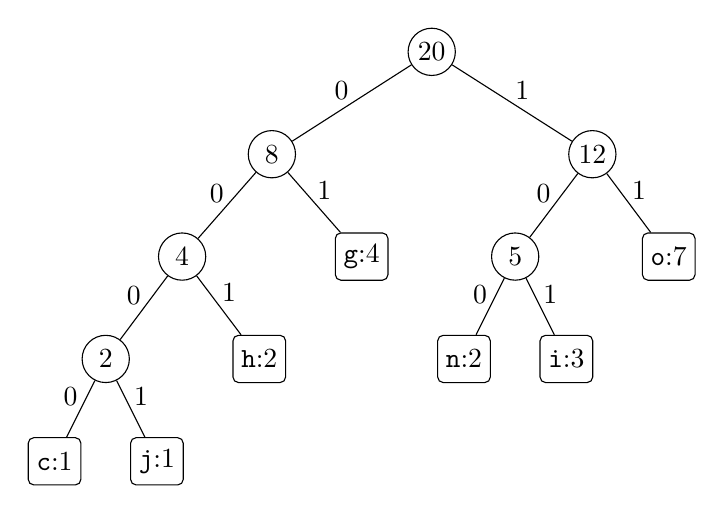
\begin{tikzpicture}[>={Stealth[length=2mm]}]
  \node[every tree node] (n0) at (4.79, 0.00) {20};
  \node[every tree node] (n1) at (2.76, -1.30) {8};
  \node[every tree node] (n2) at (1.62, -2.60) {4};
  \node[every tree node] (n3) at (0.65, -3.90) {2};
  \node[listnode] (n4) at (0.00, -5.20) {\texttt{c}:1};
  \node[listnode] (n5) at (1.30, -5.20) {\texttt{j}:1};
  \node[listnode] (n6) at (2.60, -3.90) {\texttt{h}:2};
  \node[listnode] (n7) at (3.90, -2.60) {\texttt{g}:4};
  \node[every tree node] (n8) at (6.83, -1.30) {12};
  \node[every tree node] (n9) at (5.85, -2.60) {5};
  \node[listnode] (n10) at (5.20, -3.90) {\texttt{n}:2};
  \node[listnode] (n11) at (6.50, -3.90) {\texttt{i}:3};
  \node[listnode] (n12) at (7.80, -2.60) {\texttt{o}:7};
  \draw (n3) -- node[midway, above left, inner sep=1pt] {0} (n4);
  \draw (n3) -- node[midway, above right, inner sep=1pt] {1} (n5);
  \draw (n2) -- node[midway, above left, inner sep=1pt] {0} (n3);
  \draw (n2) -- node[midway, above right, inner sep=1pt] {1} (n6);
  \draw (n1) -- node[midway, above left, inner sep=1pt] {0} (n2);
  \draw (n1) -- node[midway, above right, inner sep=1pt] {1} (n7);
  \draw (n0) -- node[midway, above left, inner sep=1pt] {0} (n1);
  \draw (n9) -- node[midway, above left, inner sep=1pt] {0} (n10);
  \draw (n9) -- node[midway, above right, inner sep=1pt] {1} (n11);
  \draw (n8) -- node[midway, above left, inner sep=1pt] {0} (n9);
  \draw (n8) -- node[midway, above right, inner sep=1pt] {1} (n12);
  \draw (n0) -- node[midway, above right, inner sep=1pt] {1} (n8);
\end{tikzpicture}
\end{center}
(c) Codewords:
\begin{center}
\begin{tabular}{|c|c|c|c|}
\hline
 Character & Frequency & Codeword & Bits \\
\hline
 \texttt{g} & 4 & \texttt{01} & 4 $\times$ 2 = 8 \\
\hline
 \texttt{o} & 7 & \texttt{11} & 7 $\times$ 2 = 14 \\
\hline
 \texttt{h} & 2 & \texttt{001} & 2 $\times$ 3 = 6 \\
\hline
 \texttt{n} & 2 & \texttt{100} & 2 $\times$ 3 = 6 \\
\hline
 \texttt{i} & 3 & \texttt{101} & 3 $\times$ 3 = 9 \\
\hline
 \texttt{c} & 1 & \texttt{0000} & 1 $\times$ 4 = 4 \\
\hline
 \texttt{j} & 1 & \texttt{0001} & 1 $\times$ 4 = 4 \\
\hline
\end{tabular}
\end{center}
(d) Huffman encoding: 51 bits. Fixed-length: 20 $\times$ 3 = 60 bits, so Huffman saves 9 bits.

(e) \texttt{00110101001100} decodes to \texttt{highn}.

\end{document}
